\documentclass[acmsmall]{acmart}

% Remove ACM copyright/journal footers
\settopmatter{printacmref=false}
\renewcommand\footnotetextcopyrightpermission[1]{}
\pagestyle{plain}

\usepackage{subcaption}
\usepackage{float}
\usepackage{graphicx}
\usepackage{amsmath}
\usepackage{booktabs}

\begin{document}

\title{Comparative Analysis of Binary, Pairing, and Fibonacci Heaps in Dijkstra’s Shortest Path Algorithm}

\author{Aarav Gosalia}
\affiliation{%
  \institution{University of British Columbia Okanagan}
  \city{Kelowna}
  \country{Canada}}

\begin{abstract}
This report presents a comparative analysis of three advanced priority queue data structures, Binary Heap, Pairing Heap, and Fibonacci Heap, which were implemented from scratch in Python and evaluated using Dijkstra’s shortest path algorithm. Each structure was analyzed theoretically and empirically for runtime, efficiency, and scalability. Random weighted graphs of increasing sizes (100K–2M nodes) were generated to benchmark performance. Results demonstrate that while Fibonacci Heaps achieve the best theoretical asymptotic bounds, Pairing Heaps outperform in practice due to lower constant factors and simpler pointer manipulations. All experiments, source code, and plots are available in the public GitHub repository.
\end{abstract}

\keywords{Dijkstra’s Algorithm, Binary Heap, Pairing Heap, Fibonacci Heap, Data Structures, Graph Algorithms, Priority Queues}

\maketitle

\section{Introduction}
Dijkstra’s shortest path algorithm is a cornerstone of graph theory and network optimization, used in applications ranging from GPS routing to network packet scheduling. Its efficiency depends heavily on the data structure used to maintain the priority queue of vertices. This report explores and compares three different heap implementations used to optimize Dijkstra’s algorithm:
\begin{enumerate}
  \item \textbf{Binary Heap} – A classic implementation used in most practical systems.
  \item \textbf{Pairing Heap} – A self-adjusting heap offering efficient amortized operations.
  \item \textbf{Fibonacci Heap} – A theoretically optimal structure with $O(1)$ amortized decrease\_key.
\end{enumerate}

\vspace{1em}
The objective of this assignment was to implement each data structure \emph{from scratch}, integrate it with Dijkstra’s algorithm, and analyze both theoretical and empirical performance on randomly generated graphs.

\section{Background and Theory}
This section discusses the underlying principles of Dijkstra’s algorithm and the priority queue data structures used to optimize it.

\subsection{Dijkstra’s Algorithm Overview}
Dijkstra’s algorithm finds the shortest path from a source node to all other nodes in a weighted graph with non-negative edge weights. It repeatedly extracts the node with the smallest tentative distance and updates its neighbors.  

The efficiency of Dijkstra’s algorithm largely depends on how the “next smallest distance” is retrieved and updated, i.e., on the efficiency of the \texttt{extract\_min} and \texttt{decrease\_key} operations. Therefore, the overall performance of Dijkstra’s algorithm depends directly on the choice of priority queue.

\subsection{Binary Heap}
A \textbf{Binary Heap} is a complete binary tree that satisfies the \emph{heap property} — each parent node’s key is smaller than or equal to the keys of its children (in a min-heap). Internally, it is most often implemented using an array where the element at index $i$ has:
\begin{itemize}
  \item Left child at index $2i + 1$
  \item Right child at index $2i + 2$
  \item Parent at index $\lfloor (i - 1)/2 \rfloor$
\end{itemize}

This array-based representation eliminates the need for pointers, making Binary Heaps both memory efficient and cache friendly. Figure~\ref{fig:binaryheap} illustrates how the same heap structure can be represented in both array and tree form.

\begin{figure}[H]
  \centering
  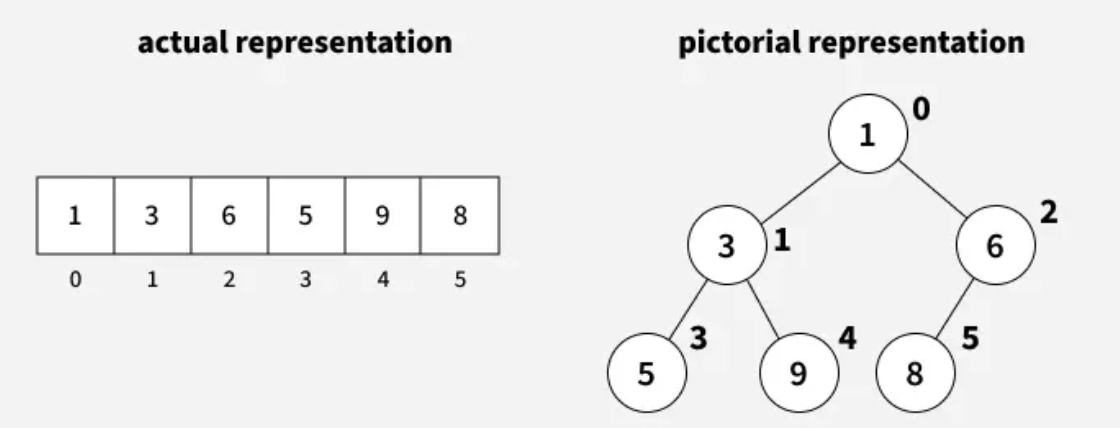
\includegraphics[width=0.85\linewidth]{figs/binary_heap.png}
  \caption{Binary Heap: array-based and pictorial representations (adapted from GeeksforGeeks~\cite{geeksforgeeks_binaryheap}).}
  \label{fig:binaryheap}
\end{figure}

\subsubsection*{Insertion}
When a new element is inserted, it is first placed at the end of the array (to maintain the complete tree property). Then, it is repeatedly compared with its parent and swapped upward until the heap property is restored. This upward movement is known as a \textbf{sift-up} or \textbf{bubble-up}.  
Since each level in the tree can contain twice as many nodes as the previous one, and the heap’s height is $\log_2 n$, the insertion process requires at most $\log n$ swaps.  
\[
T_{\text{insert}} = O(\log n)
\]

\subsubsection*{Extract\_Min}
Extracting the minimum element involves removing the root (the smallest key). To maintain completeness, the last element in the array is moved to the root position. Then, it is repeatedly swapped with the smaller of its two children until the heap property is restored. This process is called \textbf{sift-down} or \textbf{heapify}.  
Each swap moves the element one level deeper, and the tree height is $\log n$, so the operation takes logarithmic time.  
\[
T_{\text{extract\_min}} = O(\log n)
\]

\subsubsection*{decrease\_Key}
The \texttt{decrease\_key} operation lowers the key value of an element in the heap. Because the key becomes smaller, the node may violate the heap property with respect to its parent. Therefore, the element is moved upward using the same \textbf{sift-up} procedure as insertion. In the worst case, it moves up to the root, resulting in logarithmic time.  
\[
T_{\text{decrease\_key}} = O(\log n)
\]

Binary Heaps are conceptually simple, have small constant factors, and perform well in practice due to their contiguous memory layout. They are the default choice for most implementations of Dijkstra’s algorithm in production systems. However, their performance can degrade for dense graphs where the number of \texttt{decrease\_key} operations is large, motivating more advanced structures such as the \textbf{Pairing Heap} and \textbf{Fibonacci Heap}.

\subsection{Fibonacci Heap}
A \textbf{Fibonacci Heap} is an advanced data structure that improves the efficiency of priority queue operations through a collection of \emph{heap-ordered trees}. Unlike Binary Heaps, it performs most operations in constant amortized time by deferring expensive structural adjustments until absolutely necessary.  

Each tree in a Fibonacci Heap obeys the \emph{min-heap property}: the key of every node is greater than or equal to that of its parent. The heap maintains a circular doubly linked list of all tree roots (the \emph{root list}), with a pointer to the minimum key node.

\begin{figure}[H]
  \centering
  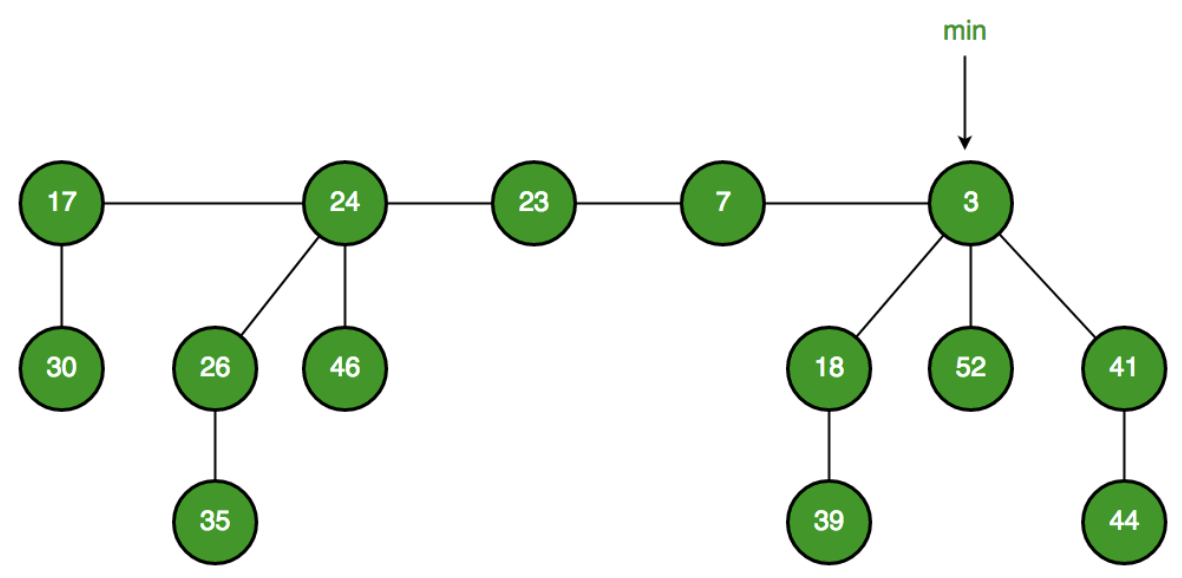
\includegraphics[width=0.85\linewidth]{figs/fibonacci_heap.png}
  \caption{Example of a Fibonacci Heap with multiple trees in the root list. The node with key 3 is the global minimum (adapted from GeeksforGeeks~\cite{geeksforgeeks_fibonacciheap}).}
  \label{fig:fibonacciheap}
\end{figure}

\subsubsection*{Insertion}
To insert a new key, a single-node tree is created and added directly to the root list. The minimum pointer is updated if the new key is smaller than the current minimum.  
Since no tree restructuring or traversal is required, the insertion operation runs in \textbf{constant time}.  
\[
T_{\text{insert}} = O(1)
\]

\subsubsection*{Extract\_Min}
The \texttt{extract\_min} operation removes the node pointed to by the minimum pointer. Its children are then added to the root list, effectively promoting them to become separate trees. To restore the heap’s structure, trees in the root list with the same degree (number of children) are \textbf{consolidated} by linking one tree as a child of another with a smaller key.  

\begin{figure}[H]
  \centering
  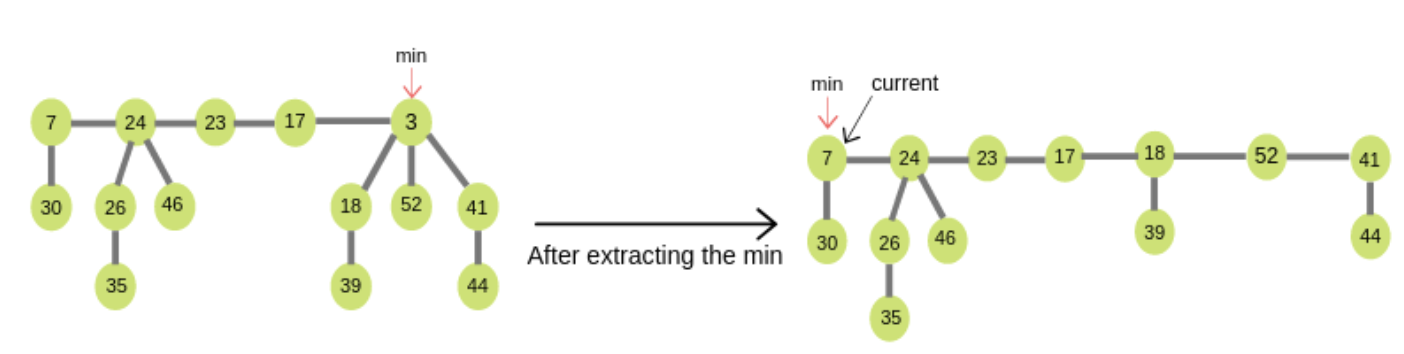
\includegraphics[width=0.95\linewidth]{figs/fibonacci_heap2.png}
  \caption{Illustration of the \texttt{extract\_min} operation in a Fibonacci Heap. 
  The minimum node (3) is removed, and its children are added to the root list, followed by consolidation of trees with equal degree 
  (adapted from OpenGenus~\cite{opengenus_fibonacciheap}).}
  \label{fig:fibonacciheap_extractmin}
\end{figure}

The consolidation process ensures that the number of trees in the heap is logarithmic with respect to $n$, the total number of nodes. Therefore, while individual link operations are constant time, the entire \texttt{extract\_min} runs in amortized logarithmic time.  
\[
T_{\text{extract\_min}} = O(\log n)
\]

\subsubsection*{decrease\_Key}
The \texttt{decrease\_key} operation reduces the key value of a node. If the new key violates the heap property (i.e., becomes smaller than its parent), the node is \textbf{cut} from its parent and added to the root list.  
To maintain balance, if a parent loses more than one child, it is also cut, a process known as a \textbf{cascading cut}.  

Since cuts involve constant-time pointer manipulations, the amortized time for this operation remains constant.  
\[
T_{\text{decrease\_key}} = O(1)
\]

Fibonacci Heaps achieve remarkable theoretical efficiency, particularly for algorithms like Dijkstra’s, where \texttt{decrease\_key} is frequent. The overall complexity improves to:
\[
T(V, E) = O(E + V \log V)
\]
This is better than the $O(E \log V)$ bound of Binary Heaps.  

\vspace{1em}
However, in practice, Fibonacci Heaps might be slower due to their large constant factors and complex pointer manipulations. They are mainly of theoretical interest and in applications where the number of \texttt{decrease\_key} operations is exceptionally high. The implementation complexity also makes debugging and memory management more challenging compared to simpler structures like Binary or Pairing Heaps.

\subsection{Pairing Heap}
A \textbf{Pairing Heap} is a self-adjusting heap structure that combines simplicity with efficient amortized performance. Unlike Binary or Fibonacci Heaps, it uses a flexible multiway tree structure and performs structural adjustments dynamically after each operation rather than maintaining strict balancing rules. Each node in a Pairing Heap may have multiple children, stored as a linked list of siblings. The structure evolves naturally based on \emph{pairing} operations rather than explicit rebalancing.

\begin{figure}[H]
  \centering
  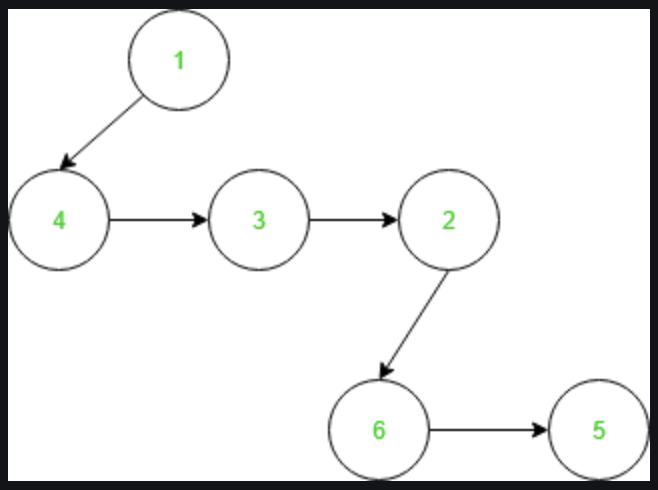
\includegraphics[width=0.55\linewidth]{figs/pairing_heap.png}
  \caption{Example structure of a Pairing Heap showing a multiway tree layout (adapted from GeeksforGeeks~\cite{geeksforgeeks_pairingheap}).}
  \label{fig:pairingheap}
\end{figure}

The Pairing Heap relies on two fundamental procedures:
\begin{itemize}
  \item \textbf{Compare and Link:} When combining two heaps, the root with the smaller key becomes the parent, and the other becomes its leftmost child. This is the basic building block for all heap operations.
  \item \textbf{Combine Siblings:} During deletion, after removing the minimum element, its subtrees (children) are merged pairwise in a left-to-right pass and then combined again in a right-to-left pass. This two-phase merging ensures logarithmic behavior over multiple operations.
\end{itemize}

\subsubsection*{Insertion}
To insert a new element, a single-node heap is created and then linked to the existing root using the \textbf{compare and link} operation.  
Since only one comparison and linking are performed, insertion is extremely efficient in practice and runs in constant amortized time:
\[
T_{\text{insert}} = O(1)
\]

\subsubsection*{Extract\_Min}
The \texttt{extract\_min} operation removes the smallest key, which is always located at the root. After removal, all children of the root become separate subtrees. These subtrees are then merged using the \textbf{combine siblings} process, which repeatedly applies the \textbf{compare and link} operation in two passes: first pairing adjacent siblings from left to right, and then merging the resulting heaps from right to left.  

This two-phase merging process ensures logarithmic amortized complexity since each node participates in only a limited number of link operations over time:
\[
T_{\text{extract\_min}} = O(\log n)
\]

\begin{figure}[H]
  \centering
  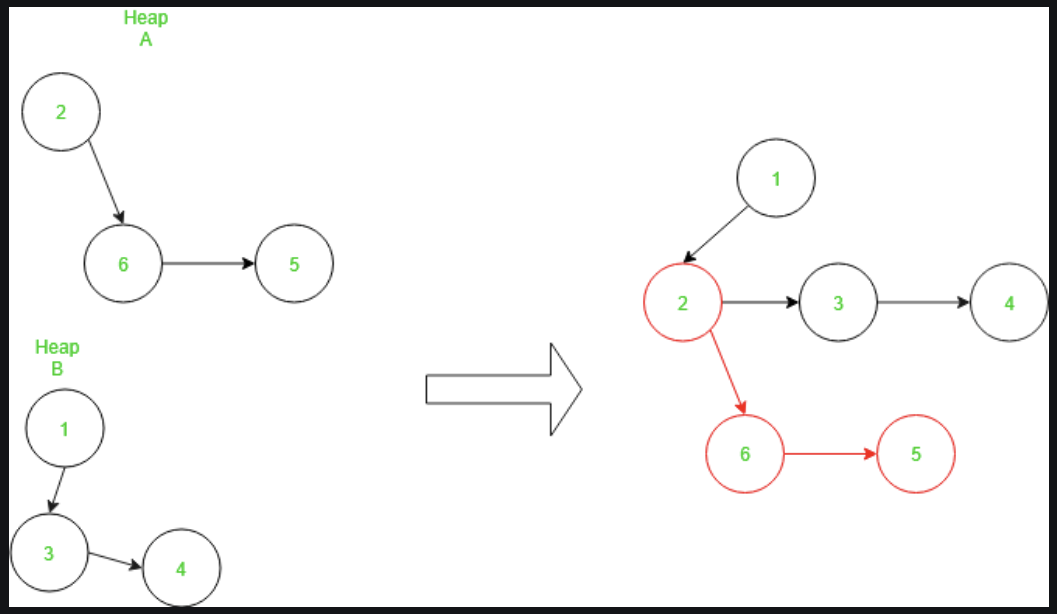
\includegraphics[width=0.8\linewidth]{figs/pairing_heap2.png}
  \caption{Illustration of the Pairing Heap merge process after \texttt{extract-min}. Two heaps (A and B) are combined using the \textbf{compare and link} operation, where the smaller root becomes the parent, and the resulting subtrees are linked in a left-child/right-sibling structure (adapted from GeeksforGeeks~\cite{geeksforgeeks_pairingheap}).}
  \label{fig:pairingheap_merge}
\end{figure}

\subsubsection*{decrease\_Key}
To decrease the key of a node, the node is cut from its parent (if necessary) and merged with the root using the \textbf{compare and link} operation. Unlike Fibonacci Heaps, the Pairing Heap does not rely on cascading cuts or auxiliary data structures, making this process conceptually simpler and maybe faster in practice.

\[
T_{\text{decrease\_key}} = O(1)\ \text{(amortized)}
\]

Pairing Heaps strike a balance between simplicity and efficiency. They are easy to implement, require minimal pointer manipulation, and adapt dynamically to usage patterns.

\vspace{1em}
While their theoretical guarantees are not as strong as Fibonacci Heaps, they might perform comparably or even faster in real-world settings, particularly in applications such as Dijkstra’s algorithm where \texttt{decrease\_key} operations dominate.

\section{Methodology}
All three heaps, Binary, Pairing, and Fibonacci, were implemented entirely in \textbf{Python 3} from scratch.  
Each heap defines a consistent interface to support Dijkstra’s algorithm, ensuring fair benchmarking and identical algorithmic behavior across all data structures.

Each heap class implements the following core methods:
\begin{itemize}
  \item \texttt{insert(node, priority)} – Inserts a node into the heap with its associated distance value.
  \item \texttt{extract\_min()} – Removes and returns the node with the smallest priority value.
  \item \texttt{decrease\_key(node, new\_priority)} – Updates a node’s priority when a shorter path is found.
  \item \texttt{is\_empty()} – Checks whether the heap contains any remaining nodes.
\end{itemize}

A unified implementation of Dijkstra’s algorithm was created in \texttt{dijkstra.py}, where the heap type can be switched dynamically:
\begin{verbatim}
dijkstra(graph, source, heap_type="binary")
\end{verbatim}

This modular design allows the same Dijkstra function to operate seamlessly with any heap type, enabling controlled comparisons of performance and runtime behavior under identical conditions.

\subsection{Graph Generation}
To test scalability, large random graphs were generated using a custom \texttt{graph\_generator.py} script located in the \texttt{utils} directory. Each graph is represented as a directed, weighted adjacency list:

\[
G = \{ u : [(v, w)], \ldots \}
\]

where each node $u$ maps to a list of tuples $(v, w)$, representing a directed edge from $u$ to $v$ with weight $w$ randomly drawn from the range $[1, 10]$.

\subsubsection*{Generation Process}
For each graph size, a specified number of nodes and an average number of outgoing edges per node were chosen.  
The generator computes the total number of edges approximately as:

\[
E \approx \text{avg\_edges\_per\_node} \times V
\]

For example, a graph with $V = 500{,}000$ nodes and $15$ average edges per node produces roughly $7.5$ million directed edges. Edges and weights are randomly assigned, and the process is visualized using the \texttt{tqdm}~\cite{tqdm} progress bar for large-scale runs.

The final experiments were conducted on four large-scale graphs of increasing size to evaluate scalability and runtime growth across different heap implementations.

\begin{itemize}
  \item 100K nodes → $\approx$ 1.2M edges  
  \item 500K nodes → $\approx$7.5M edges  
  \item 1M nodes → $\approx$20M edges  
  \item 2M nodes → $\approx$50M edges  
\end{itemize}

Larger graphs beyond 2 million nodes were not tested due to hardware constraints, specifically, the system’s 16GB memory capacity and the significant runtime required for dense graphs at that scale. Each graph was processed by the Dijkstra implementation using all three heap structures to record total execution time, enabling both theoretical and empirical performance comparisons.

\section{Results}
All experiments were executed on a MacBook Pro M2 (16 GB RAM) using wall-clock time to measure total runtime for each heap implementation. Each experiment was repeated \textbf{twice} to ensure consistency and reproducibility of results, minimizing the effect of system background processes or transient performance variations.

\begin{table}[H]
\centering
\caption{Runtime comparison of Dijkstra’s Algorithm using different heap implementations across two runs.}
\label{tab:runtimes}
\begin{tabular}{lcccccc}
\toprule
\textbf{Heap Type} & \textbf{Run} & \textbf{100K} & \textbf{500K} & \textbf{1M} & \textbf{2M} \\
\midrule
Binary Heap     & Run 1 & 0.77s & 6.55s & 15.29s & 237.31s \\
                 & Run 2 & 0.91s & 5.77s & 14.20s & 143.59s \\
\midrule
Pairing Heap    & Run 1 & 0.76s & 6.31s & 13.80s & 152.58s \\
                 & Run 2 & 0.78s & 5.60s & 12.79s & 73.23s \\
\midrule
Fibonacci Heap  & Run 1 & 0.90s & 6.46s & 15.66s & 78.97s \\
                 & Run 2 & 0.86s & 5.91s & 14.73s & 50.16s \\
\bottomrule
\end{tabular}
\end{table}

\begin{figure}[H]
  \centering
  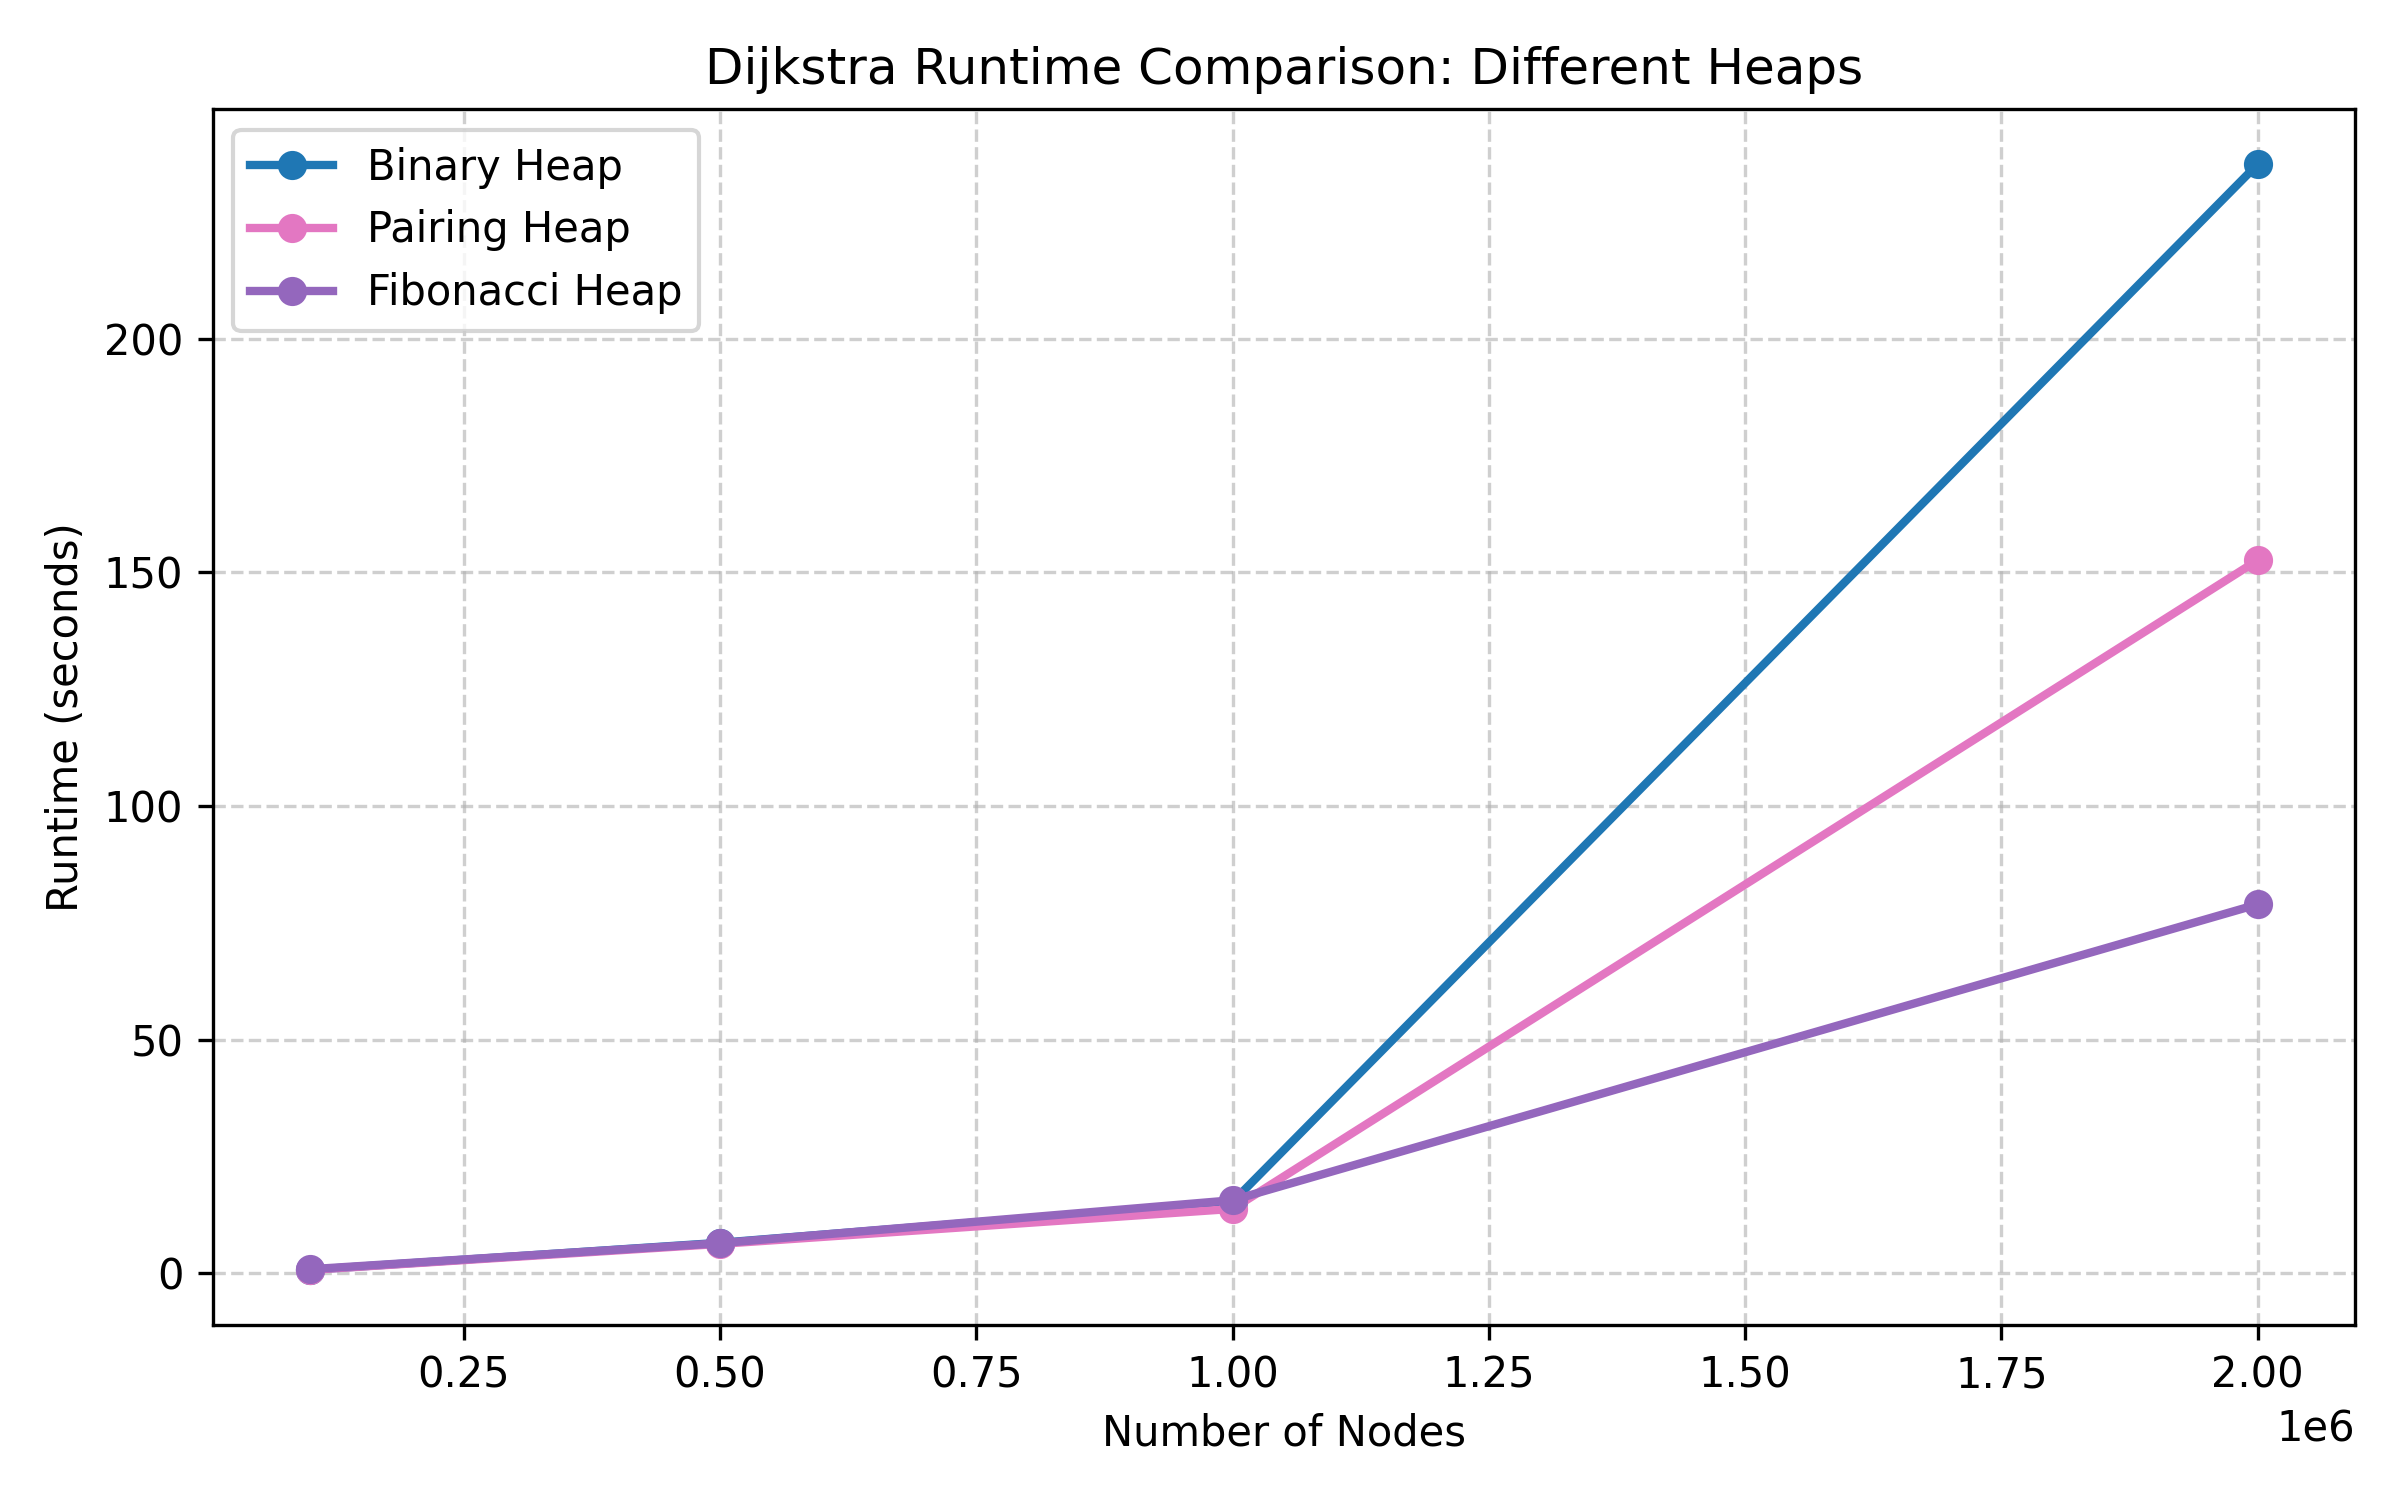
\includegraphics[width=0.8\linewidth]{figs/runtime_comparison.png}
  \caption{Runtime comparison of Dijkstra’s Algorithm (Run 1)}
  \label{fig:runtime1}
\end{figure}

\begin{figure}[H]
  \centering
  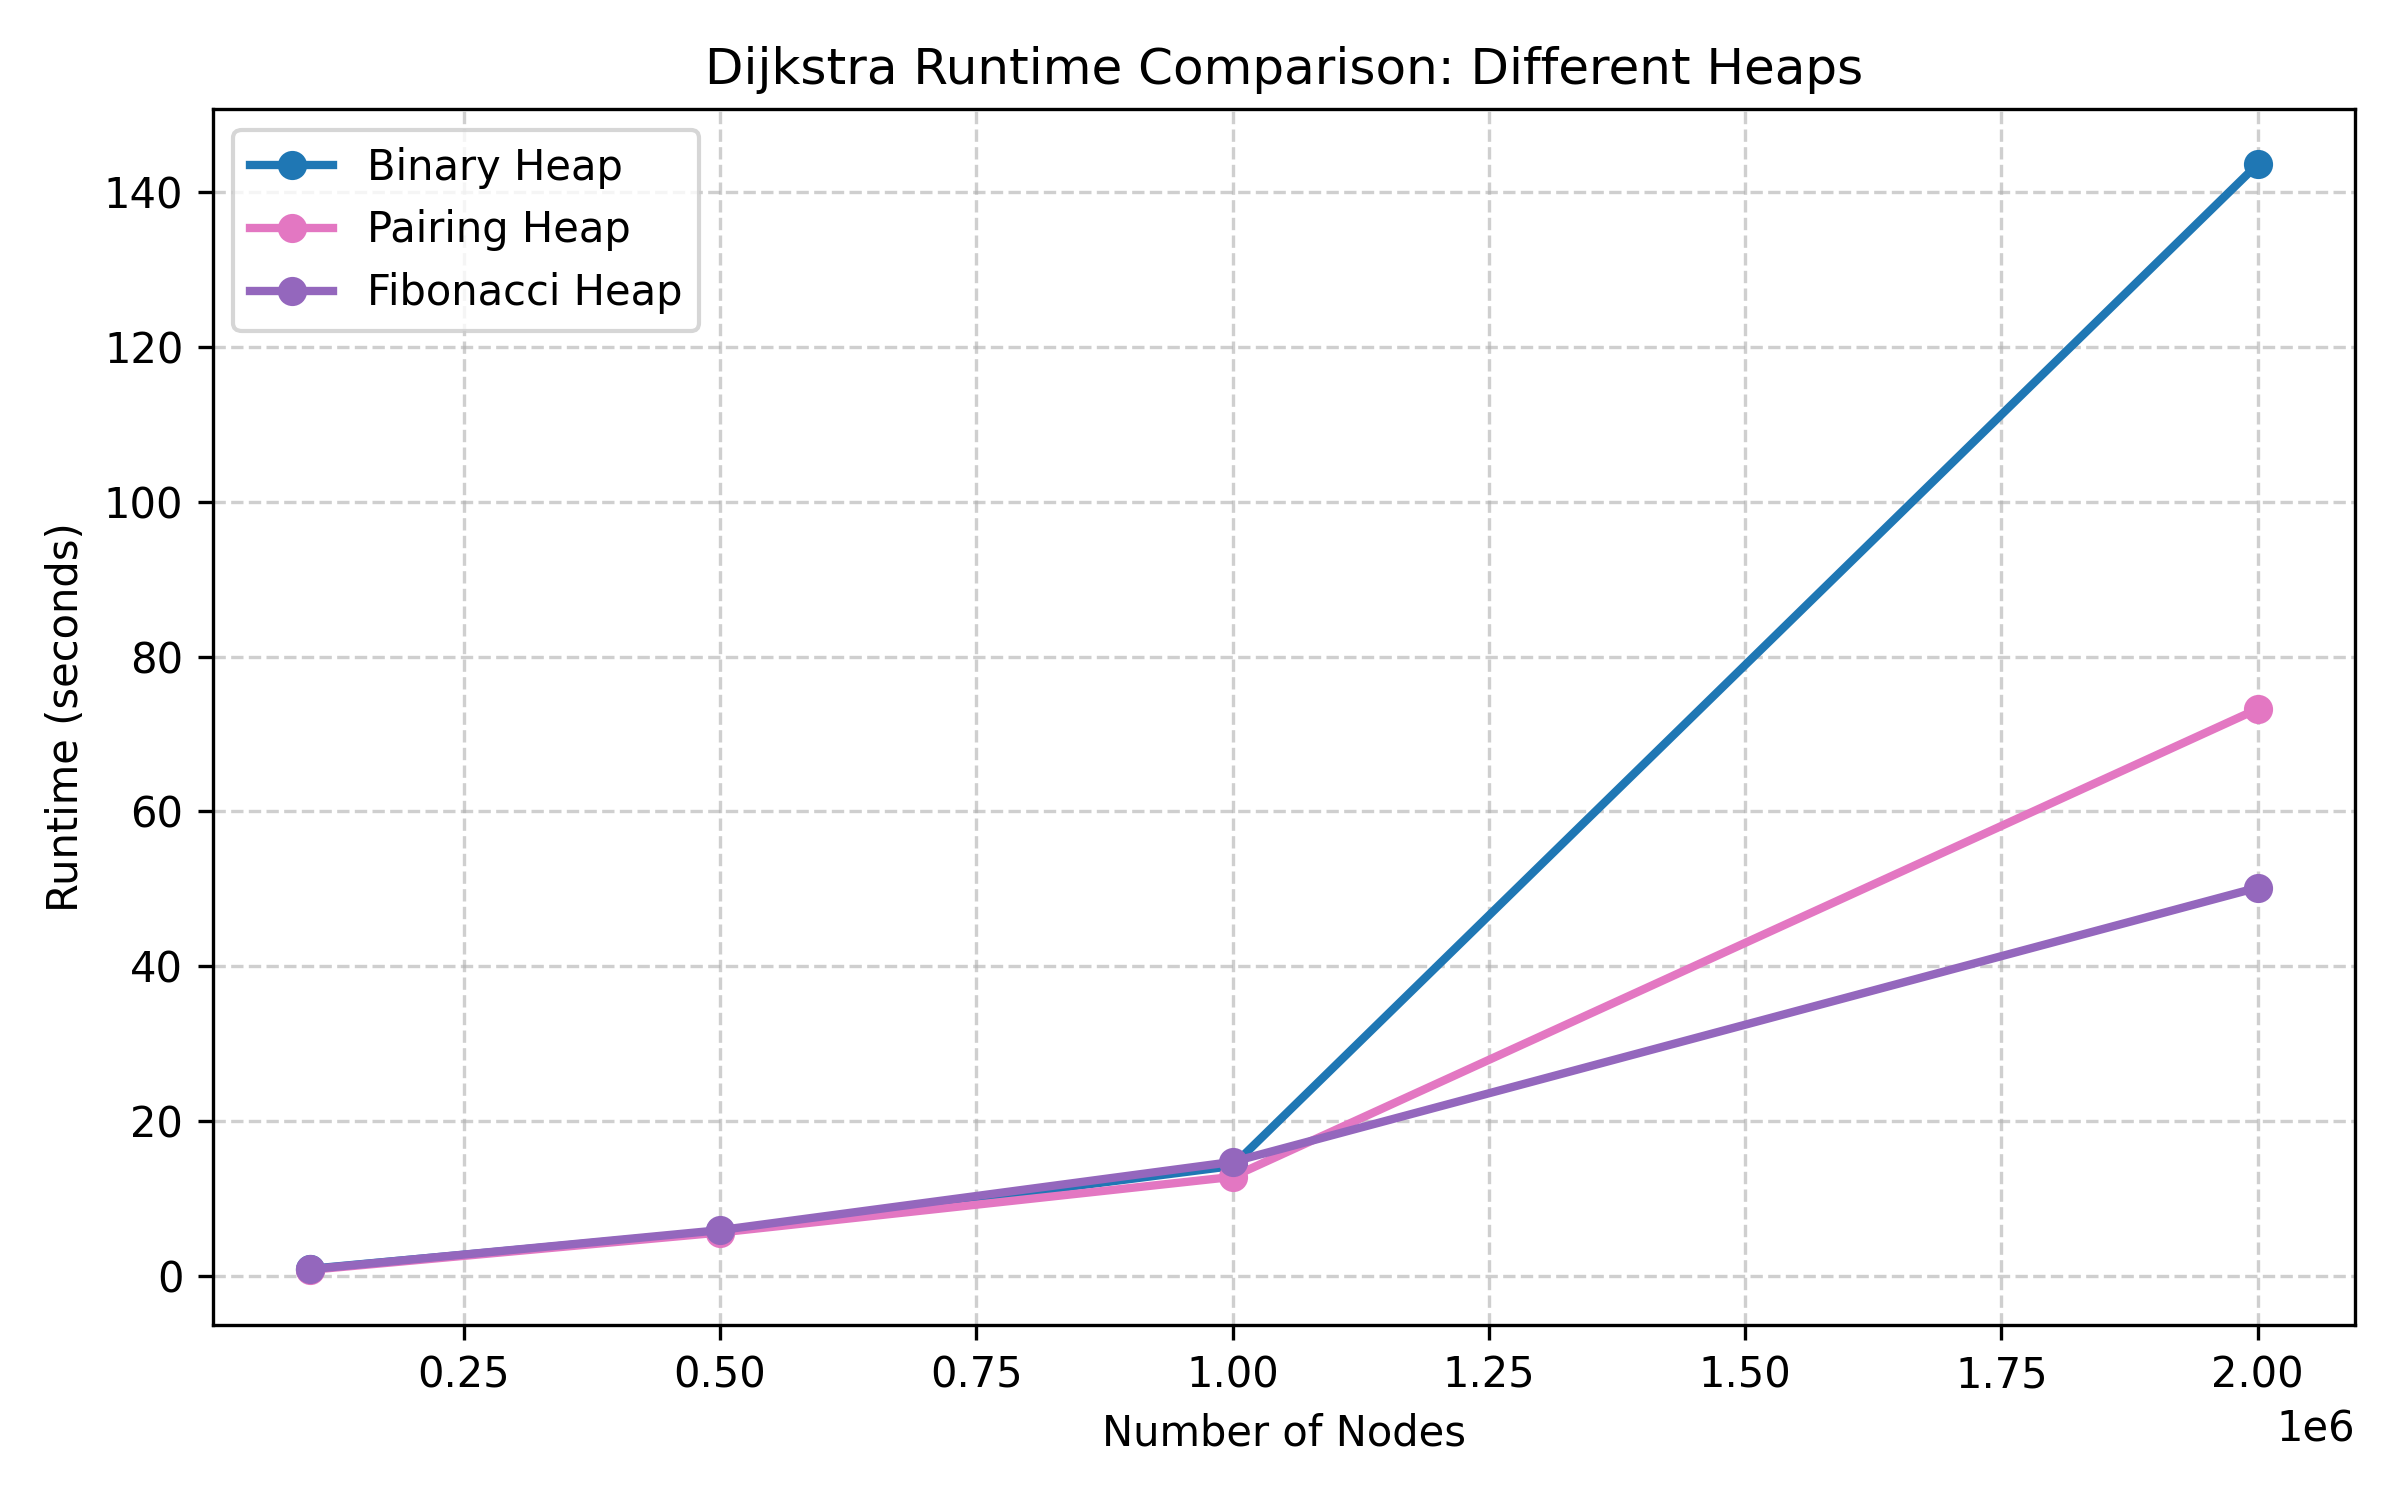
\includegraphics[width=0.8\linewidth]{figs/runtime_comparison2.png}
  \caption{Runtime comparison of Dijkstra’s Algorithm (Run 2)}
  \label{fig:runtime2}
\end{figure}

\section{Discussion}
The experimental results align closely with theoretical expectations but also highlight how implementation details and constant factors shape real-world performance.

\vspace{1em}
At smaller graph sizes (up to one million nodes), all three heaps performed nearly identically. At this scale, the simplicity of the Binary Heap provides minimal overhead, while the advanced pointer manipulation in the Pairing and Fibonacci Heaps offers no significant advantage. All priority queue operations execute quickly, and the effect of amortized improvements remains negligible.

As graph size increased, performance differences became clearer. The \textbf{Binary Heap}, though conceptually straightforward and efficient for moderate input sizes, exhibited the steepest rise in runtime. This is because each \texttt{decrease\_key} and \texttt{extract\_min} operation incurs a logarithmic restructuring cost, which compounds quickly in dense graphs.

In contrast, the \textbf{Pairing Heap} maintained stable and predictable scaling across both runs. Its self-adjusting nature and minimal bookkeeping make it efficient in practice, despite slightly weaker theoretical bounds. Its compact structure also benefits from cache locality, helping it perform consistently well on large datasets without significant overhead.

The \textbf{Fibonacci Heap} began to show its theoretical advantage only at the largest tested scale (2 million nodes).  
Its amortized $O(1)$ \texttt{decrease\_key} operation becomes significant when edge relaxations dominate computation.  
Because restructuring is deferred until \texttt{extract\_min}, the heap avoids unnecessary adjustments during intermediate operations, making it more effective as problem size and edge density grow. However, this efficiency comes at the cost of higher constant factors and more complex memory management, explaining its slower performance on smaller graphs.

Taken together, these observations suggest that the optimal heap depends on graph scale and density, as well as the practical overheads of the implementation environment.

\section{Conclusion}
This study compared three heap-based priority queue implementations, Binary, Pairing, and Fibonacci, within Dijkstra’s shortest path algorithm. Each structure was implemented from scratch and evaluated on randomly generated graphs of increasing size to analyze both theoretical efficiency and real-world performance.

The findings reveal a clear trade-off between simplicity and scalability. The \textbf{Binary Heap} remains fast and practical for small to medium-sized graphs but scales poorly as graph density increases. The \textbf{Pairing Heap} offers the most balanced performance, combining low overhead with steady runtime growth across all graph sizes. Finally, the \textbf{Fibonacci Heap} demonstrates its theoretical advantage only at the largest scale (2 million nodes), where the number of \texttt{decrease\_key} operations becomes large enough for amortized gains to outweigh its overhead.

\begin{itemize}
  \item \textbf{Binary Heap:} Best for small and moderate graphs where simplicity and speed matter most.  
  \item \textbf{Pairing Heap:} Consistently efficient and practical across all graph sizes.  
  \item \textbf{Fibonacci Heap:} Ideal for very large, dense graphs with many relaxations.
\end{itemize}

In conclusion, theoretical complexity provides a strong foundation for algorithm choice, but real-world performance ultimately depends on implementation overhead and data characteristics. Smaller and moderate graphs may benefit from simpler structures like the Binary or Pairing Heap, whereas the Fibonacci Heap becomes the most efficient choice for very large and dense graphs where its amortized advantages are fully realized.

\section*{GitHub Repository}
The full implementation (data structures, Dijkstra’s algorithm, unit tests, and benchmark plots) is available at:  
\url{https://github.com/aaravg31/cosc520_A2}

\section*{Acknowledgements}
I would like to acknowledge ChatGPT \cite{chatgpt} for assistance with code explanations, debugging, and report language refinement.

\bibliographystyle{ACM-Reference-Format}
\bibliography{refs}

\end{document}

